\section{Solar System Dynamics, Meteorites \& Cratering }\label{sec:q1}    

\subsection*{a)}
Orbital period and semi-major axis are related by:

\subsubsection*{i)}
\begin{equation}
    T = 2 \pi \sqrt{\frac{a^3}{GM}}
\end{equation}

As $GM$ is a property of the sun (heaviest body) and all planets in question orbit the sun, we do not have to compute it. We then get:

\begin{equation}
    \begin{split}
        T_{Mars} = \sqrt{a_{Mars}^3} \sqrt{(4\pi^2 GM)^{-1}} = \sqrt{1.5^3} \sqrt{(4\pi^2 GM)^{-1}} = 1.837 \sqrt{(4\pi^2 GM)^{-1}} \; \text{Earth years}\\
        T_{Jupiter} = \sqrt{a_{Jupiter}^3} \sqrt{(4\pi^2 GM)^{-1}} = \sqrt{5^3} \sqrt{(4\pi^2 GM)^{-1}} = 11.18 \sqrt{(4\pi^2 GM)^{-1}} \; \text{Earth years}\\
        T_{Saturn} = \sqrt{a_{Saturn}^3} \sqrt{(4\pi^2 GM)^{-1}} = \sqrt{9.54^3} \sqrt{(4\pi^2 GM)^{-1}} = 29.466 \sqrt{(4\pi^2 GM)^{-1}} \; \text{Earth years}
    \end{split}
\end{equation}

This leads to:

\begin{equation}
    \begin{split}
        T_{Mars} = \frac{1.837}{11.18} \cdot T_{Jupiter} = 0.16 \; \text{Jovian years} \\
        T_{Saturn} = \frac{29.466}{11.18} \cdot T_{Jupiter} = 2.64 \; \text{Jovian years} 
    \end{split}
\end{equation}

\subsubsection*{ii)}
Lagrange point L1 is the point in between two bodies where the gravity potentials of the two bodies are equal. Formally, to find this point from the Hill equations, one needs to compute where:

\begin{equation}
        \frac{\partial U}{\partial x} = \frac{\partial U}{\partial y} = \frac{\partial U}{\partial z} = 0
\end{equation}

However, since we're looking for the point in between the bodies where the gravity potentials are equal, we know that this point lies on the edge of the Hill sphere, as indicated in the figure. The radius of this sphere is:

\begin{equation}
    R_h = a \cdot \sqrt{\frac{m_q}{3(m_p+m_q)}}
\end{equation}

\begin{figure}[H]
    \centering
    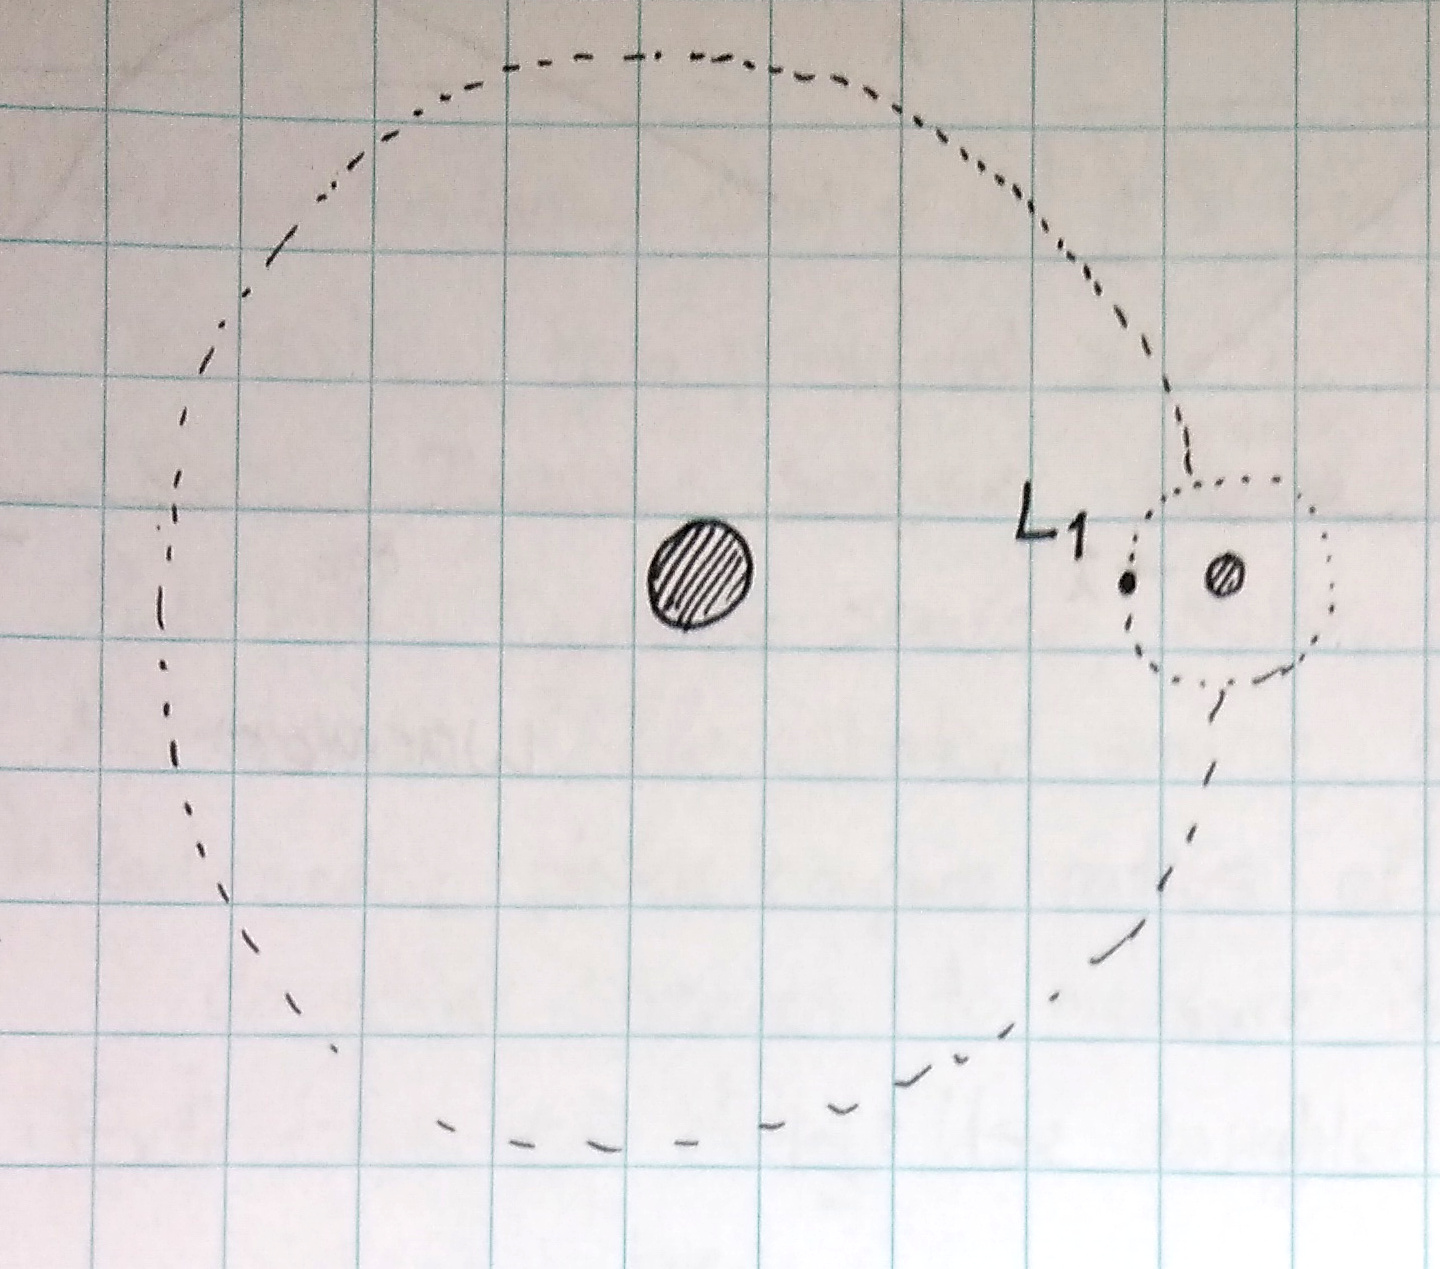
\includegraphics[width=0.5\textwidth]{figures/1b.jpg}
    %\caption{Caption}
    \label{fig:my_label}
\end{figure}


\subsubsection*{iii)}
The waves are caused by the gravitational attraction of Daphnis, which is moving faster than the material of the rings. There is a perpendicular component to this wave, as Daphnis' motion is inclined with respect to the ring-plane. This can also be seen in the figure, where a certain particle P experiences the gravitational attraction from Daphnis.

\begin{figure}[H]
    \centering
    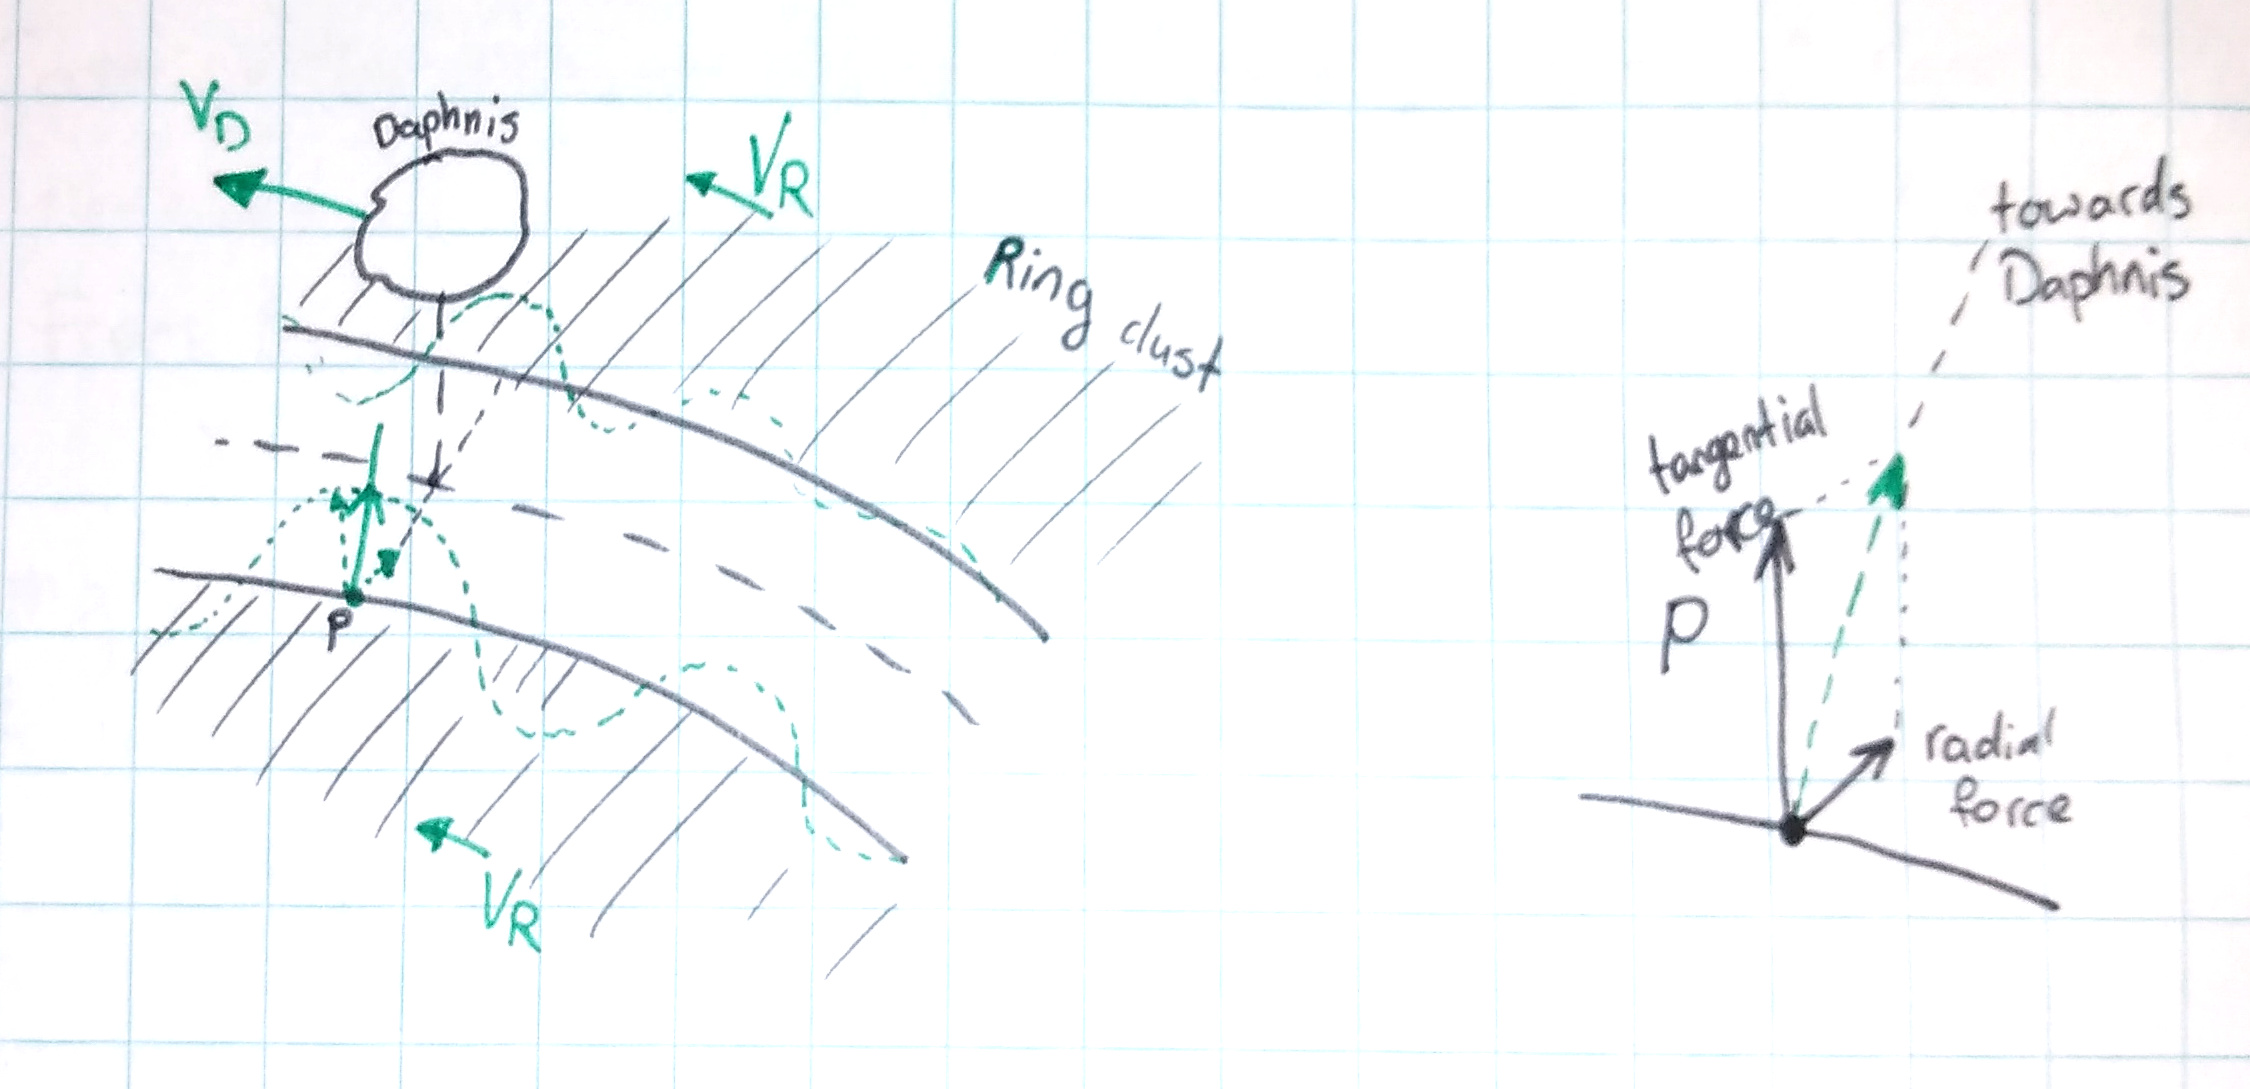
\includegraphics[width=0.8\textwidth]{figures/1biii.jpg}
    %\caption{Caption}
    \label{fig:my_label3}
\end{figure}

One can determine the density of Daphnis if one knows the volume and the mass. If one assumes a certain spheroid shape for Daphnis, and estimates the radius from imagery, one can find an approximation for the volume. From the wave properties in the image, one can find $\mu_{Daphnis}$, from which the mass of Daphnis can be obtained. The density is then the mass divided by the volume.

\subsection*{b)}
\subsubsection*{i)}
Laplace equation:
\begin{equation}
\begin{split}
        \nabla^2 U = 0 \\
        \frac{\partial^2 U}{\partial x^2} + \frac{\partial^2 U}{\partial y^2} + \frac{\partial^2 U}{\partial z^2} = 0
\end{split}
\end{equation}

For bodies of non-uniform density, there are disturbances and the potential starts embodying oscillatory behaviour, which are typically modelled using Legendre polynomials. 

\subsubsection*{ii)}
The Legendre polynomials must be known to model this, to gain insight in the nature of the disturbance.

\subsection*{c)}
\subsubsection*{i)}
The gravitational attraction of the Moon creates tidal bulges in the surface body of water on Earth. These bulges lag behind substantially compared to the motion of the Moon. This causes a net positive torque on the Moon, slightly enhancing its orbit over time.

\subsubsection*{ii)}
The effects of tidal energy dissipation are most pronounced when the orbiting moon is near its planetary host. For an eccentric orbit, this periodically occurs in the perigee, and over time the orbit will become more circular as a result.

\subsubsection*{iii)}
\textit{[PS \& SOD Reader p.223]}
\begin{enumerate}
    \item Raising of lunar orbit dissipates $0.121 \cdot 10^{12}$ W.
    \item The change of Earth's axial rotation dissipates $2.441 \cdot 10^{12}$ W.
    \item The change of the Moon's axial rotation dissipates $2.977 \cdot 10^{6}$ W.
\end{enumerate}

\textit{Editor's note: I believe that the exact values are not expected here, and that indicating the relative differences (i.e. \#2 is ~20 times as large as \#1, and \#3 is about a millionth of \#2) is sufficient.}


\subsection*{d)}
\subsubsection*{i)}
\textit{[Meteorites lecture slides - slide 16], [Lissauer - p. 286]}
\begin{enumerate}
    \item Chondritics: These are of primordial origin, typically condensed from nebulae.
    \item Irons: Igneous source, origin is molten cores of asteroids.
    \item Pallasites: Igneous source, origin is molten mantles or cores of asteroids.
    \item Achondritics: Typical origin is differentiated bodies, near the surface (i.e. crust) of asteroids or planets.
\end{enumerate}

\subsubsection*{ii)}
\begin{enumerate}
    \item Radiometric dating: Compare ratios of parent species and daughter species with a reference to estimate the age of an asteroid sample.
    \item Extinct-nuclide dating: Use daughter species products to estimate age instead. Can be used instead of radiometric dating if daughter species has fully decayed, or to obtain greater accuracy.
    \item Cosmic ray exposure dating: Determine presence of rare nuclides typical to cosmic rays in meteorite, such as $^{21}$Ne.
\end{enumerate}

\subsubsection*{iii)}
When a meteorite is entering the atmosphere of a planet, it is pulled down by its weight force, and pulled up by the atmospheric drag force. From Newton's 2nd law we know that:
\begin{equation*}
\begin{split}
    F = ma \\
    mg - \frac{1}{2} C_D \rho A V^2 = ma
\end{split}
\end{equation*}

However, at terminal velocity, we know that the velocity is constant, and therefore the acceleration equals zero:

\begin{equation*}
\begin{split}
    \frac{1}{2} C_D \rho A V_t^2 = mg\\
    V_t^2 = \frac{2 m g}{C_D \rho A}\\
    V_t = \sqrt{\frac{2 m g}{C_D \rho A}}\\
\end{split}
\end{equation*}

\subsubsection*{iv)}
A dense crater distribution implies that the body is old, given that the body features no active volcanism, tectonic activity or aggressive atmospheric erosion. Since the moon has none of these, it makes for an interesting case study, since more than half of its surface can be relatively easily mapped. The crater distribution can then be compared to the ages of the lunar rock samples brought back from the Apollo missions. 